\section{Introducci�n}

La ley de Biot y Savart nos permite calcular el campo magn�tico en un punto $P$ del espacio situado a una distancia $r$ de un conductor rectil�neo.

Las l�neas de campo son circunferencias conc�ntricas contenidas en un plano perpendicular al conductor.
El campo magn�tico $B$ en el punto $P$ tiene direcci�n tangente a las l�neas de campo y m�dulo:
\begin{equation}
    \label{eq:campo}
    B = \frac{\mu_0 I}{2\pi r}
\end{equation}

En la ecuaci�n anterior, $\mu_0$ representa la permeabilidad magn�tica del vac�o y tiene como valor $4\pi \times 10^{-7}\,$T$\cdot$m/A.

Por otro lado, el campo magn�tico terrestre es aproximadamente igual al campo generado por un dipolo magn�tico situado en el centro de la Tierra.

En un punto de latitud geogr�fica $\phi$, el campo se puede descomponer en una componente horizontal $H$ dirigida al Norte
y en una componente vertical $V$ que en el hemisferio norte est� dirigida hacia el centro de la Tierra, como se muestra en la figura~\ref{fig:earth}.

\begin{figure}[tbh!]
    \begin{center}
        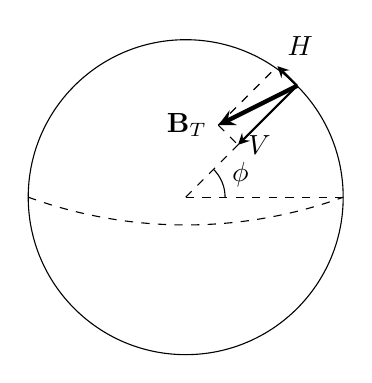
\begin{tikzpicture}

            \draw (0,0) circle (2);
            \draw[dashed] (-2,0) arc (250:290:5.85);
            \draw[dashed] (0,0) -- (2,0);
            \draw[dashed] (0,0) -- ({2*cos(45)},{2*cos(45)});
            \draw (0.5,0) arc (0:45:0.5);
            \node[] at (22.5:0.75)  {$\phi$};

            \draw[ultra thick,black,-stealth]({2*cos(45)},{2*cos(45)}) -- ++(-1,-0.5) node[anchor=east]{$\textbf{B}_T$};
            \draw[dashed] ({2*cos(45)-1},{2*cos(45)-0.5}) -- ++(0.745,0.745);
            \draw[dashed] ({2*cos(45)-1},{2*cos(45)-0.5}) -- ++(0.25,-0.25);

            \draw[thick,black,-stealth]({2*cos(45)},{2*cos(45)}) -- ++(-0.25,0.25) node[anchor=south west]{$H$};
            \draw[thick,black,-stealth]({2*cos(45)},{2*cos(45)}) -- ++(-0.75,-0.75) node[anchor=west]{$V$};

        \end{tikzpicture}
        \caption{Componentes horizontal $H$ y vertical $V$ en las que se puede descomponer el campo magn�tico terrestre $\textbf{B}_T$.}
        \label{fig:earth}
    \end{center}
\end{figure}


